\documentclass[a4j,twoside,openright,11pt]{jarticle}
%
\usepackage{amsmath,amssymb}
\usepackage{bm}
\usepackage{graphicx}
\usepackage{ascmac}
\usepackage{listliketab}
\usepackage{url}
\usepackage{listings}

\setlength{\textwidth}{15.92cm}
\setlength{\oddsidemargin}{0mm}
\setlength{\evensidemargin}{0mm}
\setlength{\topmargin}{-1cm}
\setlength{\textheight}{23.5cm}
\setlength{\footskip}{18mm}

%
\pagestyle{plain}
\begin{document}

\begin{screen}
\huge
\begin{center}
{\bf 数値解析法 第4課題}\\
\end{center}

\normalsize
\begin{flushright}
九州工業大学 機械知能工学科 機械知能コース 3年 坂本 悠作\\学籍番号 13104069 \hspace{0.2in}提出日 2015年5月19日
\end{flushright}
\end{screen}

\section{問題}
\begin{equation}
\frac{d^2y}{dx^2}+\frac{dy}{dx} + 8y = 0 
\end{equation}
上の方程式をRunge-Kutta法で解け。ただし、初期条件として次を与える。
\begin{itemize}
\item $x_0$=0のとき、$y_0=0.5$
\item $\frac{dy}{dx_0}=1$
\end{itemize}
結果はxy平面に図示せよ。
\section{解答}
初期条件により、加速度の初期条件も計算できる。
\begin{equation}
\frac{d^2y}{dx^2} = -5
\end{equation}
この条件を使って、微分方程式を積分すると、次式のようになる。
\begin{equation}
\frac{dy}{dx}+y+8xy+Cosnt=0
\end{equation}
初期条件により$C=-1.5$
\begin{equation}
\frac{dy}{dx}=1.5-y-8xy
\end{equation}
これにより、ルンゲクッタ法により値を求めていくと、図1のようになる。
また、今回は表計算ソフトを用いて計算したので、その計算過程を参考資料として添付する。今回は微小ステップhを0,01とした。
\begin{figure}[htbp]
\begin{center}
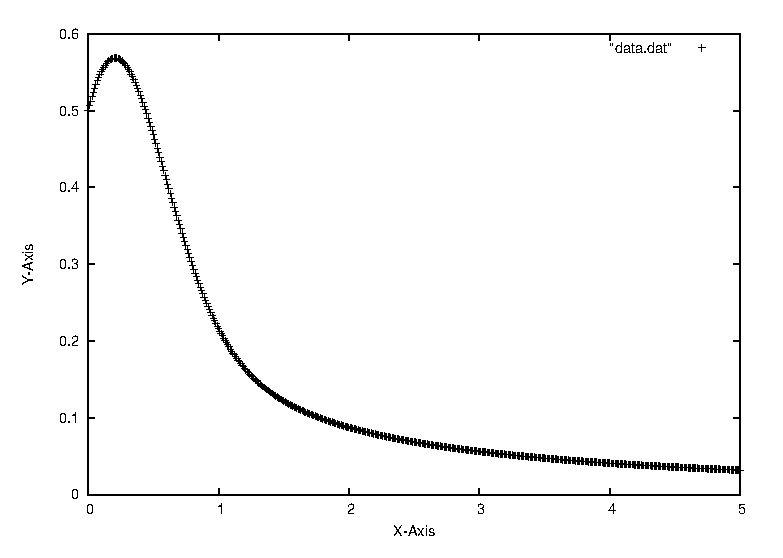
\includegraphics[width=14cm]{data.eps}
\end{center}
\caption{ルンゲクッタ法による解(y)}
\end{figure}

\end{document}